\documentclass[11pt,a4paper]{article}

\usepackage{amsmath}
\usepackage{amssymb}
\usepackage{amsthm}
\usepackage{mathtools}
\usepackage{enumerate}
\usepackage[T1]{fontenc}
\usepackage[hidelinks]{hyperref}
\usepackage{natbib}
\usepackage{xfrac}
\usepackage{caption}
\usepackage{threeparttable}
\usepackage{graphicx}
\usepackage{listings}
\usepackage{tikz}
\usetikzlibrary{automata,positioning}
\usepackage{subcaption}

\usepackage[french]{babel}
\usepackage[utf8]{inputenc}

\newtheorem{prop}{Proposition}
\newtheorem{lemma}{Lemme}
\newtheorem{thm}{Théorème}
\newtheorem{definition}{Définition}
\newtheorem{conj}{Conjecture}

\title{À propos du problème de finitude des groupes d'automates biréversibles}
\author{Maxime Flin \& Tristan François}

\begin{document}
\maketitle

\section*{Introduction}
Les automates de Mealy sont une extension des automates qui écrivent des mots en même temps qu'ils en lisent sur ce même alphabet. À partir de l'action de ces automates sur l'ensemble des mots, on peut dégager une structure de (semi-)groupe engendré par l'automate. Pour étudier cette classe de (semi-)groupes on peut travailler sur des constructions spécifiques à la structure sous-jacente d'automate (comme la minimisation ou la dualisation) pour résoudre des problèmes d'algèbre de la théorie des groupes.

Le problème de théorie des groupes auquel nous nous intéressons ici le problème de finitude, c'est-à-dire savoir si le groupe engendré par un automate de Mealy donné est fini ou non. C'est un problème difficile\footnote{trouver un truc à dire sur gillibert}, indécidable en général pour les semi-groupes d'automates. Picantin et Klimann~\cite{DBLP:journals/corr/abs-1105-4725} on proposé la $\mathfrak{md}$-réduction, une procédure alternant minimisation et dualisation de l'automate pour décider de la finitude du groupe. Klimann~\cite{Klimann13} a réussi à montrer que les groupes engendrés par des automates biréversibles à deux états ou deux lettres sont finis si et seulement si l'automate se $\mathfrak{md}$-réduit à l'automate trivial.

Nous cherchons à étendre ce résultat à tous les automates biréversibles de plus de deux lettres mais il n'est pas valide pour les automates à 4 états et 3 lettres (voir les quatres contres-exemples figure \ref{fig:fantastiques}). Cependant M. Picantin a remarqué que ces automates se factorisent et que l'automate obtenu en inversant les deux termes de la factorisation est quant à lui $\mathfrak{md}$-trivial. Nous nous sommes basés sur cet exemple pour fonder la conjecture \ref{conj:birev-mdc} qui a fait tout l'objet de notre recherche.\footnote{reformuler ?}

Pour tenter d'infirmer ou de se convaincre de la justesse de cette conjecture nous avons à la fois fait un travail théorique pour se convaincre de son bien fondé (sections \ref{sec:action} et \ref{sec:cloture}) et en même temps avons été amenés à imaginer et implémenter des techniques efficaces pour engendrer des classes d'automates qui nous intéressent (section \ref{sec:gen}) et les factoriser (section \ref{sec:facto}) -- question sur laquelle aucun vrai résultat n'existe encore. À partir de ces résultats nous avons ensuite essayé de déterminer si la $\mathfrak{mdc}$-réduction fournit un bon critère de finitude pour des classes d'automates biréversibles plus grandes (section \ref{sec:finitude}).

\section{Automates de Mealy}

\subsection{Automates de Mealy et quelques constructions}

La notion d'automate de Mealy étend la simple notion d'automate en lui ajoutant une sortie en écriture.

\begin{definition}
  Un \textbf{automate de Mealy} est la donné d'un quadruplet $\left(\mathcal{Q}, \Sigma, \delta, \rho\right)$ où $\mathcal{Q}$ est l'ensemble des états de l'automate, $\Sigma$ l'alphabet sur lequel l'automate agit, $\delta$ une famille d'applications de $\mathcal{Q}$ dans $\mathcal{Q}$ indexées par $\Sigma$ qui représente les transitions entre les états et $\rho$ une famille d'applications de $\Sigma$ dans $\Sigma$ indexées par $\mathcal{Q}$ qui représente l'écriture en sortie de l'automate.
\end{definition}

La figure \ref{fig:example} montre une machine de Mealy qui incrémente un entier écrit en binaire. Une flèche du type $p\overset{x|y}{\rightarrow}q$ indique que quand on est dans l'état $p$ et qu'on lit la lettre $x$, on se déplace dans l'état $q$ et on écrit la lettre $y$.

\begin{figure}[h]
  \begin{center}
    \begin{tikzpicture}[shorten >=1pt,node distance=2cm,on grid,auto]
      \node[state] (q_0) {$0$};
      \node[state] (q_1) [right=of q_0] {$1$};
      \path[->]
      (q_0) edge [loop above] node {$1|0$} (q_0)
      edge node {$0|1$} (q_1)
      (q_1) edge [loop above] node {$0|0~1|1$} (q_1);
    \end{tikzpicture}
    \caption{une machine de Mealy $\mathcal{A}$\label{fig:example}}
  \end{center}
\end{figure}

On peut représenter l'action d'un automate de Mealy par son diagramme en croix:

\begin{figure}[h]
  \begin{center}
    \begin{tikzpicture}
      \draw[->] (-1.25, 0.5) node[above] {1} to (-1.25, -0.5) node[below] {0};
      \draw[->] (-1.5, 0) node[left] {0} to (-1, 0) node[right] {0};

      \draw[->] (-0.25, 0.5) node[above] {0} to (-0.25, -0.5) node[below] {1};
      \draw[->] (-0.5, 0) to (0, 0) node[right] {1};

      \draw[->] (0.75, 0.5) node[above] {1} to (0.75, -0.5) node[below] {1};
      \draw[->] (0.5, 0) to (1, 0) node[right] {1};
    \end{tikzpicture}
    \caption{action de l'état 0 de la machine $\mathcal{A}$ sur le mot 101. Sont représentés horizontalement les états sucessifs et verticalement l'action de chacun de ces états sur les lettres du mot.}
  \end{center}
\end{figure}

Une autre représentation qui sera commode dans la partie \ref{sec:gen} est de le représenter par un graphe en hélice. On représente l'automate par un graphe dont les sommets sont étiquettés par des couples états lettres. Pour chaque flèche du type $p\overset{x|y}{\rightarrow}q$ dans l'automate, il y a une flèche de l'état $p, x$ vers l'état $q, y$ dans le graphe en hélice. Aussi remarque-t'on que de chaque sommets du graphe en hélice part exactement une flèche.

\begin{figure}[h]
  \begin{center}
    \begin{tikzpicture}[shorten >=1pt,node distance=2cm,on grid,auto]
      \node[state] (q_00) {$0, 0$};
      \node[state] (q_11) [right=of q_00] {$1, 1$};
      \node[state] (q_10) [above=of q_11] {$1, 0$};
      \node[state] (q_01) [above=of q_00] {$0, 1$};
      \path[->]
      (q_00) edge node {} (q_11)
      (q_10) edge node {} (q_01)
      (q_11) edge [loop right] node {} (q_11)
      (q_01) edge node {} (q_00);
    \end{tikzpicture}
    \caption{graphe en hélice de $\mathcal{A}$}
  \end{center}
\end{figure}

\begin{definition}
  Soit $\mathcal{A}=\left(\mathcal{Q}, \Sigma, \delta, \rho\right)$ un automate de Mealy.
  \begin{enumerate}[(i)]
  \item On dit que $\mathcal{A}$ est \textbf{inversible} si $\rho_q$ est une permutation de $\Sigma$ pour tout état $q\in\mathcal{Q}$.
  \item On dit que $\mathcal{A}$ est \textbf{réversible} si $\delta_x$ est une permuration de $\mathcal{Q}$ pour toute lettre $x\in\Sigma$.
  \end{enumerate}
\end{definition}

\begin{definition}
  Si un machine de Mealy $\mathcal{M}$ est inversible, alors on peut construire sont \textbf{\textit{inverse}}, noté $\mathcal{M}^{-1}$, en remplacant les flèches $p\overset{x|y}{\rightarrow}q$ par $p^{-1}\overset{y|x}{\rightarrow}q^{-1}$.
\end{definition}


\begin{figure}[h!]
  \begin{subfigure}[b]{0.5\textwidth}
    \centering
    \begin{tikzpicture}[shorten >=1pt,node distance=2cm,on grid,auto]
      \node[state] (p) {$p$};
      \node[state] (q) [right=of q_0] {$q$};
      \path[->]
      (p) edge [loop left] node {$1|0$} (p)
      (p) edge [bend left] node {$0|1$} (q)
      (q) edge [bend left] node {$0|0$} (p)
      (q) edge [loop right] node {$1|1$} (q);
    \end{tikzpicture}
  \end{subfigure}
  ~
  \begin{subfigure}[b]{0.5\textwidth}
    \centering
    \begin{tikzpicture}[shorten >=1pt,node distance=2cm,on grid,auto]
      \node[state] (p) {$p^{-1}$};
      \node[state] (q) [right=of q_0] {$q^{-1}$};
      \path[->]
      (p) edge [loop left] node {$0|1$} (p)
      (p) edge [bend left] node {$1|0$} (q)
      (q) edge [bend left] node {$0|0$} (p)
      (q) edge [loop right] node {$1|1$} (q);
    \end{tikzpicture}
  \end{subfigure}
  \caption{Automate et son inverse}
\end{figure}


\begin{definition}
  Si une machine de Mealy est réversible, alors on peut construire sont \textbf{\textir{dual}}, noté $\mathfrak{d}\mathcal{M}$, en remplacant les flèches $p\overset{x|y}{\rightarrow}q$ par $x\overset{p|q}{\rightarrow}y$.
\end{definition}


\begin{figure}[h!]
  \begin{subfigure}[b]{0.5\textwidth}
    \centering
    \begin{tikzpicture}[shorten >=1pt,node distance=2cm,on grid,auto]
      \node[state] (p) {$p$};
      \node[state] (q) [right=of p] {$q$};
      \path[->]
      (p) edge [loop left] node {$1|0$} (p)
      (p) edge [bend left] node {$0|1$} (q)
      (q) edge [bend left] node {$0|0$} (p)
      (q) edge [loop right] node {$1|1$} (q);
    \end{tikzpicture}
  \end{subfigure}
  ~
  \begin{subfigure}[b]{0.5\textwidth}
    \centering
    \begin{tikzpicture}[shorten >=1pt,node distance=2cm,on grid,auto]
      \node[state] (p) {$0$};
      \node[state] (q) [right=of p] {$1$};
      \path[->]
      (p) edge [loop left] node {$q|p$} (p)
      (p) edge [bend left] node {$p|q$} (q)
      (q) edge [bend left] node {$q|q$} (p)
      (q) edge [loop right] node {$p|p$} (q);
    \end{tikzpicture}
  \end{subfigure}
  \caption{Automate et son dual}
\end{figure}


\begin{definition}
  On dit que $\mathcal{A}$ est \textbf{biréversible} s'il est inversible, réversible et que son inverse est réversible.
\end{definition}

\begin{definition}
  Soit $\mathcal{A}=\left(\mathcal{Q}, \Sigma, \delta, \rho\right)$ un automate de Mealy. \textbf{L'équivalence de Nérode} $\equiv$ sur $\mathcal{Q}$ est la limite de la suite de relations d'équivalence $\equiv_k$ de plus en plus fines définies récursivement par

  \begin{align*}
    \forall p, q \in Q,\\
    p \equiv_0 q &\iff \rho_p = \rho_q \\
    \forall k \geq 0, p \equiv_{k+1}q &\iff \left(p\equiv_kq \wedge \forall x \in \Sigma,~\delta_x(p)=\delta_x(q)\right)
  \end{align*}

  Le \textbf{minimisé} de $\mathcal{A}$ est l'automate $\mathfrak{m}(\mathcal{A})=\left(\sfrac{\mathcal{Q}}{\equiv}, \Sigma, \bar{\delta}, \bar{\rho}\right)$, où pour tout $p\in\mathcal{Q}$ et $x\in\Sigma$, $\bar{\delta}_x(\bar{p}) = \bar{\delta_x(p)}$ et $\bar{\rho}_{\bar{p}} =  \rho_p$.
\end{definition}

\begin{definition}
  \label{def:produit}
  Soient $\mathcal{A} = \left(\mathcal{Q}, \Sigma, \delta, \rho\right)$ et $\mathcal{B} = \left(\mathcal{Q'}, \Sigma, \delta', \rho'\right)$ deux automates sur le même alphabet. On appelle \textbf{\textit{automate produit}} la machine $\mathcal{AB} = \left(\mathcal{Q}\times\mathcal{Q'}, \Sigma, \delta'', \rho''\right)$ avec

\[ \delta_x''(p_0, p_1) = (\delta_x(p), \delta_{\rho_{p_0}(x)}'(q))\]
et
\[ \rho_{(p_0,p_1)}(x) = \rho_{p_1}'(\rho_{p_0}(x)). \]
\end{definition}

\begin{figure}[h!]
  \begin{subfigure}[b]{0.5\textwidth}
    \centering
    \begin{tikzpicture}
      \draw [->] (-0.5, 1) node[left] {$p_0$} to (0.5, 1) node[right] {$q_0$};
      \draw [->] (0, 1.5) node[above] {$x$} to (0, 0.5);

      \draw [->] (-0.5, -0.5) node[left] {$p_1$} to (0.5, -0.5) node[right] {$q_1$};
      \draw [->] (0, 0) node[above] {$z$} to (0, -1) node[below] {$y$};
    \end{tikzpicture}
    \caption{En haut l'automate $\mathcal{A}$ et en bas $\mathcal{B}$}
  \end{subfigure}
  ~
  \begin{subfigure}[b]{0.5\textwidth}
    \centering
    \begin{tikzpicture}
      \draw [->] (-0.5, 0) node[left] {$p_0p_1$} to (0.5, 0) node[right] {$q_0q_1$};
      \draw [->] (0, 0.5) node[above] {$x$} to (0, -0.5) node[below] {$y$};
    \end{tikzpicture}
    \caption{Une flèche de l'automate $\mathcal{AB}$}
  \end{subfigure}
  \caption{Correspondance entre les flèches dans $\mathcal{AB}$ et celles de $\mathcal{A}$ et de $\mathcal{B}$}
\end{figure}

\begin{definition}
  La $\mathfrak{md}$-réduction...
\end{definition}

\begin{figure}[h!]
  TODO schema md-red...
  \caption{$\mathfrak{md}$-réduction de l'automate xx}
\end{figure}

\subsection{Action sur les mots et (semi-)groupes engendrés\label{sec:action}}

\subsubsection*{Notations}
Soit $\Sigma$ un alphabet. On note $\Sigma^*$ l'ensemble des mots sur cet alphabet et $\varepsilon$ le mot vide.

\begin{definition}
  Soit $\mathcal{A}=\left(\mathcal{Q}, \Sigma, \delta, \rho\right)$ un automate de Mealy. On peut étendre l'ensemble de définition de $\rho$ à $\Sigma^*$ par induction comme suit.

  Soient $p\in\mathcal{Q}$, $x\in\Sigma$ et $\textbf{u}\in\Sigma^*$
  \begin{align*}
    &\rho_p(\epsilon)=\varepsilon \\
    &\rho_p(x\textbf{u})=\rho_p(x)\rho_{\delta_x(p)}(\textbf{u})
  \end{align*}

  On définit le \textbf{semi-groupe d'automate engendré par $\mathcal{A}$} comme
  \begin{equation*}
    \left<\mathcal{A}\right>_+=\left<\rho_p, \forall p\in\mathcal{Q}\right>
  \end{equation*}

  Si l'automate $\mathcal{A}$ est inversible, alors on peut aussi considérer l'inverse des $\rho_p$. Dans ce cas, l'automate engendre un groupe noté $\left<\mathcal{A}\right>$.

\end{definition}

\begin{prop}{\cite{DBLP:journals/corr/abs-1105-4725}}
  \label{prop:finitude-d}
  Soit $\mathcal{A}$ un automate de Mealy. Le (semi-)groupe $\left<\mathcal{A}\right>_+$ est fini si et seulement si $\left<\mathfrak{d}\mathcal{A}\right>_+$ est fini.
\end{prop}

\begin{prop}
  \label{prop:finitude-m}
  Soit $\mathcal{A}$ un automate de Mealy, alors
  \[ \left<\mathfrak{m}\mathcal{A}\right> = \left<\mathcal{A}\right>. \]
\end{prop}

Des propositions \ref{prop:finitude-d} et \ref{prop:finitude-m} on déduit les propositions suivantes.

\begin{prop}
  \label{prop:md-trivial}
  Un automate de Mealy engendre un groupe fini si et seulement si son $\mathfrak{md}$-réduit engendre un groupe fini.
\end{prop}

\begin{prop}
  Tout automate $\mathfrak{md}$-trivial engendre un groupe fini.
\end{prop}

La réciproque est fausse en général. exemple ? \footnote{``un mot sur la faible efficacité en dehors des biréversibles''}

Il semble pourtant que dans la classe particulière des automates biréversibles, la $\mathfrak{md}$-réduction est efficace.

\begin{thm}{\cite{Klimann13}}
  \label{thm:K}
  Tout automate à deux lettres et/ou deux états engendre un groupe fini si et seulement s'il est $\mathfrak{md}$-trivial.
\end{thm}

Ce théorème n'est pas valide pout les automates biréversibles en général.

\begin{center}
  \begin{figure}[h]
    \makebox[\textwidth][c]{
      \begin{tikzpicture}[scale=0.65]

        \coordinate (A) at (-10,-2);
        \coordinate (B) at (-6,-2);
        \coordinate (C) at (-6,2);
        \coordinate (D) at (-10,2);
        \node[draw,circle,minimum width = 2.5em] (QA) at (A) {};
        \node[draw,circle,minimum width = 2.5em] (QB) at (B) {};
        \node[draw,circle,minimum width = 2.5em] (QC) at (C) {};
        \node[draw,circle,minimum width = 2.5em] (QD) at (D) {};
        \draw[->,>=latex] (QA) to[out=240,in=210,looseness=8] node[midway, below left]{$1|2$} (QA);
        \draw[->,>=latex] (QA) to[bend right] node[midway, below]{$0|1$} (QB);
        \draw[->,>=latex] (QA) to[bend right] node[midway, right]{$2|0$} (QD);
        \draw[->,>=latex] (QB) to[bend right] node[midway, above]{$0|0$} (QA);
        \draw[->,>=latex] (QB) to[out=330, in=300, looseness=8] node[midway, below right]{$1|2$} (QB);
        \draw[->,>=latex] (QB) to[bend right] node[midway, right]{$2|1$} (QC);
        \draw[->,>=latex] (QC) to[bend right] node[midway, left]{$2|0$} (QB);
        \draw[->,>=latex] (QC) to[out=30, in=60, looseness=8] node[midway, above right]{$0|2$} (QC);
        \draw[->,>=latex] (QC) to[bend right] node[midway, above]{$1|1$} (QD);
        \draw[->,>=latex] (QD) to[bend right] node[midway, left]{$2|1$} (QA);
        \draw[->,>=latex] (QD) to[bend right] node[midway, below]{$1|0$} (QC);
        \draw[->,>=latex] (QD) to[out=120, in=150, looseness=8] node[midway, above left]{$0|2$} (QD);


        \coordinate (A) at (0,0);
        \coordinate (B) at (0:3);
        \coordinate (C) at (120:3);
        \coordinate (D) at (240:3);
        \node[draw,circle,minimum width = 2.5em] (QA) at (A) {};
        \node[draw,circle,minimum width = 2.5em] (QB) at (B) {};
        \node[draw,circle,minimum width = 2.5em] (QC) at (C) {};
        \node[draw,circle,minimum width = 2.5em] (QD) at (D) {};
        \draw[->,>=latex] (QA) to[bend right] node[midway, below]{$1|0$} (QB);
        \draw[->,>=latex] (QB) to[bend right] node[midway, above]{$2|0$} (QA);
        \draw[->,>=latex] (QA) to[bend right] node[midway, above right]{$0|1$} (QC);
        \draw[->,>=latex] (QC) to[bend right] node[midway, below left]{$0|2$} (QA);
        \draw[->,>=latex] (QA) to[bend right] node[midway, above left]{$2|2$} (QD);
        \draw[->,>=latex] (QD) to[bend right] node[midway, below right]{$1|1$} (QA);
        \draw[->,>=latex] (QB) to[bend right] node[midway, below]{$1|2$} (QC);
        \draw[->,>=latex] (QC) to[bend left=40] node[midway, above]{$2|1$} (QB);
        \draw[->,>=latex] (QC) to[bend right] node[midway, right]{$1|0$} (QD);
        \draw[->,>=latex] (QD) to[bend left=40] node[midway, left]{$2|0$} (QC);
        \draw[->,>=latex] (QD) to[bend right] node[midway, above]{$0|2$} (QB);
        \draw[->,>=latex] (QB) to[bend left=40] node[midway, below]{$0|1$} (QD);

        \coordinate (A) at (6,-2);
        \coordinate (B) at (10,-2);
        \coordinate (C) at (10,2);
        \coordinate (D) at (6,2);
        \node[draw,circle,minimum width = 2.5em] (QA) at (A) {};
        \node[draw,circle,minimum width = 2.5em] (QB) at (B) {};
        \node[draw,circle,minimum width = 2.5em] (QC) at (C) {};
        \node[draw,circle,minimum width = 2.5em] (QD) at (D) {};
        \draw[->,>=latex] (QA) to[out=240,in=210,looseness=8] node[midway, below left]{$1|0$} (QA);
        \draw[->,>=latex] (QA) to[bend right] node[midway, below]{$0|2$} (QB);
        \draw[->,>=latex] (QA) to[bend right] node[midway, right]{$2|1$} (QD);
        \draw[->,>=latex] (QB) to[bend right] node[midway, above]{$0|2$} (QA);
        \draw[->,>=latex] (QB) to[out=330, in=300, looseness=8] node[midway, below right]{$1|1$} (QB);
        \draw[->,>=latex] (QB) to[bend right] node[midway, right]{$2|0$} (QC);
        \draw[->,>=latex] (QC) to[bend right] node[midway, left]{$2|0$} (QB);
        \draw[->,>=latex] (QC) to[out=30, in=60, looseness=8] node[midway, above right]{$0|1$} (QC);
        \draw[->,>=latex] (QC) to[bend right] node[midway, above]{$1|2$} (QD);
        \draw[->,>=latex] (QD) to[bend right] node[midway, left]{$2|1$} (QA);
        \draw[->,>=latex] (QD) to[bend right] node[midway, below]{$1|2$} (QC);
        \draw[->,>=latex] (QD) to[out=120, in=150, looseness=8] node[midway, above left]{$0|0$} (QD);
      \end{tikzpicture}
    }
    \caption{Les plus petits contre-exemples à une généralisation du théorème \ref{thm:K}, aka Les 4 fantastiques. Le quatrième est l'inverse du premier.\label{fig:fantastiques}}
  \end{figure}
\end{center}

Ces contre-exemples sont pourtant factorisables, et en conjugant\footnote{mauvaise formulation, conjugaison non introduite} leur factorisation, on trouve un automate $\mathfrak{md}$-trivial. Ce qui conduit à la conjecture suivante.

\begin{figure}
  TODO: illustrer mdc red sur un fantastique
  \caption{$\mathfrak{mdc}$-réduction de xx}
\end{figure}

\begin{conj}
  \label{conj:birev-mdc}
  Un automate de Mealy biréversible engendre un groupe fini si et seulement si son $\mathfrak{mdc}$-réduit est trivial\footnote{pas compris}.
\end{conj}

Cette conjecture est l'objet des recherches ménées au cours de ce projet.

\begin{prop}
  \label{prop:finitude-c}
  Soient $\mathcal{A}, \mathcal{B}$ des automates de Mealy.
  L'automate $\mathcal{A}\mathcal{B}$ engendre un groupe fini si et seulement si $\mathcal{B}\mathcal{A}$ engendre un groupe fini.
\end{prop}

\begin{proof}
  Soient $\mathcal{A}=\left(\mathcal{Q}_1, \Sigma, \delta, \rho\right)$ et $\mathcal{B}=\left(\mathcal{Q}_2, \Sigma, \delta, \rho\right)$ des automates de Mealy sur un même alphabet.

  On suppose sans perte de généralité $\mathcal{Q}_1$ et $\mathcal{Q}_2$ disjoints. On écrit donc $\rho$ pour les deux automates sans ambiguïté.

  On suppose $\left<\mathcal{A}\mathcal{B}\right>$ fini.

  Tout élément de $\left<\mathcal{B}\mathcal{A}\right>$ est de la forme
  \[
    \rho_{p_1q_1}\circ\rho_{p_2q_2}\circ\cdots\circ\rho_{p_nq_n}
  \]
  où les $p_i$ sont des éléments de $\mathcal{Q}_2$ et les $q_i$ des éléments de $\mathcal{Q}_1$. Or
  \begin{align*}
    \rho_{p_1q_1}\circ\rho_{p_2q_2}\circ\cdots\circ\rho_{p_nq_n} &= \rho_{q_1}\circ\rho_{p_1}\circ\rho_{q_2}\circ\rho_{p_2}\circ\cdots\circ\rho_{q_n}\circ\rho_{p_n} \\
    &=\rho_{q_1}\circ\left(\rho_{p_1}\circ\rho_{q_2}\circ\rho_{p_2}\circ\cdots\circ\rho_{q_n}\right)\circ\rho_{p_n} \\
    &=\rho_{q_1}\circ\underbrace{\left(\rho_{q_2p_1}\circ\rho_{q_3p_2}\circ\cdots\circ\rho_{q_np_{n-1}}\right)}_{\in\left<\mathcal{A}\mathcal{B}\right>}\circ\rho_{p_n}
  \end{align*}

  On en déduit que tout élément de $\left<\mathcal{B}\mathcal{A}\right>$ s'écrit comme la composition d'un $\rho_{q},~q\in\mathcal{Q}_1$, d'un $\rho_\bullet\in\left<\mathcal{A}\mathcal{B}\right>$ et d'un $\rho_{p},~p\in\mathcal{Q}_2$. Or $\mathcal{Q}_1$ et $\mathcal{Q}_2$ sont finis, donc le nombre de choix de $p$ et de $q$ est fini. De plus, on a supposé le nombre d'éléments $\rho_\bullet\in\left<\mathcal{A}\mathcal{B}\right>$ fini, donc le nombre d'élements qui s'écrivent \[ \rho_q\circ\rho_\bullet\circ\rho_p \] est fini. On a montré plus haut que tout élément de $\left<\mathcal{B}\mathcal{A}\right>$ sont de cette forme, on en conclut qu'il y en a un nombre fini.

  Les facteurs $\mathcal{A}$ et $\mathcal{B}$ jouant des rôles complètement symétriques, la même démonstration marche pour montrer la réciproque.
\end{proof}

On remarque toutefois que cette proposition n'est pas vraie pour les produits $\mathcal{ABC}$ et $\mathcal{ACB}$.

\begin{figure}[h!]
  CONTRE EXEMPLE
  \caption{Contre-exemple pour 3 facteurs}
\end{figure}

On déduit des propositions \ref{prop:finitude-d}, \ref{prop:finitude-m} et \ref{prop:finitude-c} une des implications de la conjecture~\ref{conj:birev-mdc}.

\begin{prop}\footnote{wtf ?}
  Tout automate de Mealy engendre un (semi)groupe fini si et seulement si son $\mathfrak{mdc}$-réduit engendre un (semi)groupe fini.
\end{prop}

\section{Génération et factorisation d'automates de Mealy}
La génération de biréversibles et la factorisation d'automates de Mealy sont des problèmes pour lesquels aucune solution efficace n'existe pour l'instant. Dans le but de pouvoir infirmer ou consolider la conjecture \ref{conj:birev-mdc}, une partie de notre travail a été d'essayer de trouver et d'implémenter des méthodes de génération et de factorisation efficaces pour les automates de Mealy biréversibles.


\subsection{Clôture de classes d'automates\label{sec:cloture}}

Puisque nous nous interéssons à la classe des automates biréversibles, montrons qu'elle est bien close par les opérations qui nous interéssent, \emph{i.e.} la dualisation, la minimisation, le produit et la factorisation.

\begin{prop}[Clôture des inversibles par produit]
  Soient $\mathcal{A}$ et $\mathcal{B}$ des automates de Mealy \textbf{inversibles}. Alors $\mathcal{A}\cdot\mathcal{B}$ est inversible
\end{prop}

\begin{proof}
  Soient $\mathcal{A}=\left(\mathcal{Q}, \Sigma, \delta, \rho\right)$ et $\mathcal{B}=\left(\mathcal{Q'}, \Sigma, \delta', \rho'\right)$ deux automates inversibles, et soit $\mathcal{A\cdot B}=\left(\mathcal{Q\times Q'}, \Sigma, \delta'', \rho''\right)$ leur produit.


  Considérons un état $(p, r)$ de ce produit. Alors $\rho_r\circ\rho'_p=\rho_{(p,r)}$, or puisque les automates $\mathcal{A}$ et $\mathcal{B}$ sont inversibles, $\rho_p$ et $\rho'_r$ sont des permutations du groupe de symétrie de $\Sigma$, on en déduit que $\rho_{(p, r)}$ en est une aussi.

  On a bien que tous les ${(\rho''_q)}_{q\in Q\times Q'}$ sont des permutations sur les lettres, c'est à dire que l'automate est inversible.
\end{proof}

\begin{prop}[Clôture des réversibles par produit]
  Soient $\mathcal{A}$ et $\mathcal{B}$ des automates de Mealy \textbf{réversibles}. Si $\mathcal{A}$ est \textbf{inversible}, alors $\mathcal{A}\cdot\mathcal{B}$ est réversible.
\end{prop}

\begin{proof}
  Soient $\mathcal{A}=\left(\mathcal{Q}, \Sigma, \delta, \rho\right)$ et $\mathcal{B}=\left(\mathcal{Q'}, \Sigma, \delta', \rho'\right)$ deux automates réversibles, et soit $\mathcal{A\cdot B}=\left(\mathcal{Q\times Q'}, \Sigma, \delta'', \rho''\right)$ leur produit.


  On suppose $\mathcal{A}$ inversible.


  Par définition $\delta''_x(pr)=(\delta_x(p), \delta'_{\rho_p(x)}(r))$. Or, puisque les automates sont réversibles, les $(\delta_x)_{x\in\Sigma}$ et ${(\delta'_x)}_{x\in\Sigma}$ sont des bijections. De plus, $\mathcal{A}$ est inversible donc les ${(\rho_p)}_{p\in \mathcal{Q}}$ sont des bijections. On en conclut que les ${(\delta''_{pr})}_{pr\in\mathcal{Q}\times\mathcal{Q'}}$ sont aussi des bijections.
\end{proof}

Les biréversibles ne sont pas clôs par produit.

\begin{figure}
  CONTRE EXEMPLE
  \caption{Deux automates biréversibles dont le produit ne l'est pas.}
\end{figure}

\begin{prop}[Clôture des inversibles par facteur]\label{prop_cloture_inv_facteurs}
  Soit $\mathcal{A}$ un automate de Mealy \textbf{inversible} qui se factorise en deux automates $\mathcal{A}_1$ et $\mathcal{A}_2$. Alors ces deux automates sont aussi inversibles.
\end{prop}

Avant de faire la démonstration, rappelons un résultat élémentaire qui nous sera utile.
\begin{lemma}\label{lem:bij}
  Soit $f:A\rightarrow B$ et $g:B\rightarrow C$ deux fonctions telles que $g\circ f$ soit une bijection.
  Alors
  \begin{enumerate}[(i)]
  \item $g$ est surjective
  \item $f$ est injective.
  \end{enumerate}
\end{lemma}

\begin{proof}
  \begin{enumerate}[(i)]
  \item Soit $x\in C$, alors il existe un $y\in A$ tel que
    \[ (g\circ f)(y) = x \]
    c'est à dire tel que
    \[ g(f(y)) = x. \]
    On en déduit immédiatement que $g$ est surjective.

  \item Soit $x,y \in B$ tels que \[ f(x) = f(y). \] Alors \[ g(f(x)) = g(f(y)) \] et on en déduit que $x = y$, c'est à dire que $f$ est injective.
  \end{enumerate}
\end{proof}

\begin{proof}[Démonstration de la proposition \ref{prop_cloture_inv_facteurs}]
  Soient $\mathcal{A}=\left(\mathcal{Q\cdot Q'}, \Sigma, \delta, \rho\right)$, $\mathcal{A}_1=\left(\mathcal{Q}, \Sigma, \delta', \rho'\right)$ et $\mathcal{A}_2=\left(\mathcal{Q'}, \Sigma, \delta'', \rho''\right)$ tel que ci dessus.

  Pour chaque état $(p, r)$ de $\mathcal{A}$, $\rho_{(p, r)}\in \mathfrak{S}(\Sigma)$. Comme $\mathcal{A}=\mathcal{A}_1\cdot\mathcal{A}_2$, on a l'égalité $\rho_{(p, r)}=\rho'_r\circ\rho''_p$.

  Or $\rho_{(p, r)}$ est une bijection donc $\rho'_r$ est sujective et $\rho''_p$ est injective (lemme \ref{lem:bij}). Or puisque ce sont des fonctions de $\Sigma$ dans $\Sigma$ qui est fini on a l'équivalence
  \[ injective \iff surjective \iff bijective. \]
  D'où le résultat.
\end{proof}

\begin{prop}\label{prop_inverse_produit}
    Soit $\mathcal{A}$ un automate de Mealy \textbf{inversible} qui se factorise en deux automates $\mathcal{A}_1$ et $\mathcal{A}_2$.
    Alors $\mathcal{A}^{-1} = \mathcal{A}_2^{-1} \cdot \mathcal{A}_1^{-1}$.
\end{prop}

\begin{proof}
  Notons $\rho$, $\rho_1$ et $\rho_2$ les fonctions associées aux machines $\mathcal{A}$, $\mathcal{A}_1$ et $\mathcal{A}_2$. Alors par définition \[ \rho = \rho_2\circ\rho_1 \] et donc que \[ \rho^{-1} = \left(\rho_2\circ\rho_1\right)^{-1} = \rho_1^{-1}\circ\rho_2^{-1}. \]

  $\rho_1^{-1}$ et $\rho_2^{-1}$ sont bien définies puisqu'on a montré précedémment (prop \ref{prop_cloture_inv_facteurs}) que les automates inversibles étaient clos par facteurs.
\end{proof}

\begin{prop}[Clôture des réversibles par facteur]\label{prop_cloture_rev_facteurs}
  Soit $\mathcal{A}$ un automate de Mealy \textbf{réversible} qui se factorise en deux automates $\mathcal{A}_1$ et $\mathcal{A}_2$. Alors
  \begin{itemize}
  \item $\mathcal{A}_1$ est réversible.
  \item si $\mathcal{A}_1$ est inversible, alors $\mathcal{A}_2$ est réversible.
  \end{itemize}
\end{prop}

\begin{proof}
  Soient $\mathcal{A}=\left(\mathcal{Q\cdot Q'}, \Sigma, \delta, \rho\right)$ réversible, $\mathcal{A}_1=\left(\mathcal{Q}, \Sigma, \delta', \rho'\right)$ et $\mathcal{A}_2=\left(\mathcal{Q'}, \Sigma, \delta'', \rho''\right)$ tels que $\mathcal{A} = \mathcal{A}_1\cdot\mathcal{A}_2$.

  Par définition, on a que $\delta_x(pr) = (\delta'_x(p), \delta''_{\rho'_p(x)}(r))$. Les ${(\delta_x)}_{x\in\Sigma}$ sont inversibles, alors il est clair les ${(\delta'_x)}_{x\in\Sigma}$ sont inversibles.

  De plus, chacun des $\delta''_{\rho_p(x)}$ est inversibles, donc si $\mathcal{A}_1$ est inversible, les ${(\rho_p)}_{p\in\Sigma}$ étant des bijections, alors tous les ${(\delta''_x)}_{x\in\Sigma}$ sont inversibles. D'où $\mathcal{A}_2$ est réversible.
\end{proof}

\begin{prop}[Clôture des biréversibles par facteurs]
  Soit $\mathcal{A}$ un automate \textbf{biréversible} et $\mathcal{A}_1$, $\mathcal{A}_2$ des automates tels que $\mathcal{A}=\mathcal{A}_1\cdot\mathcal{A}_2$, alors $\mathcal{A}_1$ et $\mathcal{A}_2$ sont biréversible.
\end{prop}

\begin{proof}
    $\mathcal{A}$ est biréversible, donc en particulier $\mathcal{A}$ est inversible et réversible. D'après la proposition \ref{prop_cloture_inv_facteurs}, $\mathcal{A}_1$ et $\mathcal{A}_2$ sont inversibles. Puisque $\mathcal{A}_1$ est inversible, d'après la proposition \ref{prop_cloture_rev_facteurs}, $\mathcal{A}_1$ et $\mathcal{A}_2$ sont réversibles.

    D'après la proposition \ref{prop_inverse_produit}, $\mathcal{A}^{-1} = \mathcal{A}_2^{-1} \cdot \mathcal{A}_1^{-1}$. Or $\mathcal{A}^{-1}$ est réversible puisque $\mathcal{A}$ est biréversible. Donc, toujours d'après la proposition \ref{prop_cloture_rev_facteurs} et puisque $\mathcal{A}_1^{-1}$ est inversible, $\mathcal{A}_1^{-1}$ et $\mathcal{A}_2^{-1}$ sont réversibles.

    Ainsi, $\mathcal{A}_1$ et $\mathcal{A}_2$ sont bien biréversibles.
\end{proof}

\subsection{Algorithme de génération des biréversibles\label{sec:gen}}

\subsubsection*{Représentation des machines de Mealy en mémoire}
Les machines de Mealy sont représentés en mémoire par deux matrices \lstinline$delta$ et \lstinline{rho}, l'une représentant les $(\delta_x)_{x\in\Sigma}$ et l'autre les $(\rho_p)_{p\in\mathcal{Q}}$. Dans les deux cas les lignes des matrices sont indexées par les états et les colonnes par les lettres.

\begin{enumerate}[(i)]
\item On reconnait une machine réversible en vérifiant que les colonnes de \textrm{delta}  sont des permutations.
\item On reconnait une machine inversible en vérifiant que les lignes dans \textrm{rho} sont des permutations.
\end{enumerate}

\subsubsection*{L'algorithme}
Notre algorithme de génération se base sur le résultat suivant

\begin{prop}{\cite{DBLP:journals/corr/abs-1105-4725}}
  \label{thm:ir-helix}
  Soit $\mathcal{A}$ un automate de Mealy inversible réversible. Les propositions suivantes sont équivalentes~:

  \begin{enumerate}[(i)]
  \item $\mathcal{A}$ est biréversible
  \item Le graphe en hélice de $\mathcal{A}$ est une union de cycles disjoints.
  \end{enumerate}
\end{prop}

Notre algorithme procède donc à la recherche exhaustive de toutes les machines de Mealy inversibles réversibles en maintenant la contrainte que le graphe en hélice est une union de cycles disjoints.

Nous maintenons une liste de \textit{sources} et de \textit{cibles} qui représentent les sommets du graphe en hélice desquels encore aucune flèche ne part et les sommets du graphe en hélice vers lesquels encore aucune flèche ne pointe. En choisissant nos sommets dans ces ensembles nous nous assuront que le graphe en hélice obtenu est bien une union de cycles disjoints. À chaque fois que nous modifions \textrm{delta} ou \textrm{rho}, nous vérifions que la machine est bien inversible-réversible.

Ainsi, les automates trouvés -- en vertu de la proposition \ref{thm:ir-helix} -- sont bien biréversibles. La structure globale du programme est représentée sur la figure~\ref{fig:gen-pseudo-code}

\begin{figure}
\begin{verbatim}
def rec(start, prev, sources, targets, delta, rho):
    if not sources and not targets:
        # plus de sources ni de targets
        # on a fini la génération et on retourne l'automate
        return delta, rho

    # s'il n'y a pas de précédent on commence un nouveau cycle
    # alors on choisit un sommets dans les sources
    # et on commence un nouveau cycle
    if not prev:
        start = sources.pop()

    [...]

    # on backtrack sur les targets
    for _ in range(len(targets)):
        # on choisit le sommet suivant dans le cycle
        # puis on modifie l'automate en conséquence
        p_next, x_next = targets.pop(0)
        delta[p_prev][x_prev] = p_next
        rho[p_prev][x_prev] = x_next

        [...]
        # on s'assure que l'automate est encore
        # inversible-réversible et si c'est le cas
        # on lance la récursion pour explorer cette direction
        if valid_delta(delta) and valid_rho(rho):
          res = rec(...)

    [...]

\end{verbatim}
  \caption{Structure globale de la fonction de génération en python\label{fig:gen-pseudo-code}}
\end{figure}

\subsubsection*{À isomorphisme près}

On a rapidement constaté que le nombre d'automates à générer est très important. Aussi, il ne semble pas réaliste de tester la $\mathfrak{mdc}$-réduction sur tous ceux-ci. On a donc cherché à extraire seulement les classes d'isomorphismes au sens de Nérode de notre génération.

La bibliothèque de graphe \textrm{Nauty}~\cite{Nauty} est une des plus efficaces. Il a fallu s'assurer que les morphismes de \textit{graphe} trouvé par \textrm{Nauty} correspondent bien à des morphismes de \textit{machine de Mealy}. Nous avons donc utilisé ce que nous appellons \textit{\textbf{le graphe en hélice augmenté}}: le graphe en hélice auquel nous ajoutons des sommets pour chaque état et chaque lettre de l'automate et les relions à ceux qu'ils étiquettent. Ainsi, si un morphisme de graphe trouvé par Nauty permute deux lettres ou deux états, il les permute sur tous les sommets du graphe en hélice.

\begin{figure}[h]\label{fig:helix-aug}
  \begin{center}
    \begin{tikzpicture}[scale=0.7]
        \coordinate (A) at (-10, 0);
        \coordinate (B) at (-7, 0);

        \node[draw,circle,minimum width = 2.5em] (q_0) at (A) {$a$};
        \node[draw,circle,minimum width = 2.5em] (q_1) at (B) {$b$};
        \path[->]
        (q_0) edge [loop left] node {$0|1$} (q_0)
        (q_0) edge [bend left] node[midway, above] {$1|1$} (q_1)
        (q_1) edge [bend left] node[midway, below] {$0|0$} (q_0)
        (q_1) edge [loop right] node {$1|0$} (q_1);

        %############################################

        \coordinate (A) at (-1,-1);
        \coordinate (B) at (1,-1);
        \coordinate (C) at (1,1);
        \coordinate (D) at (-1,1);

        \coordinate (P1) at (-3,0);
        \coordinate (P2) at (3,0);
        \coordinate (PA) at (0,-3);
        \coordinate (PB) at (0,3);

        \node[draw,circle,minimum width = 2.5em] (QA) at (A) {$0|a$};
        \node[draw,circle,minimum width = 2.5em] (QB) at (B) {$1|a$};
        \node[draw,circle,minimum width = 2.5em] (QC) at (C) {$1|b$};
        \node[draw,circle,minimum width = 2.5em] (QD) at (D) {$0|b$};

        \node[draw,circle,minimum width = 2.5em,fill=black!20!green] (F1) at (P1) {$0$};
        \node[draw,circle,minimum width = 2.5em,fill=black!20!green] (F2) at (P2) {$1$};
        \node[draw,circle,minimum width = 2.5em,fill=white!20!orange] (FA) at (PA) {$a$};
        \node[draw,circle,minimum width = 2.5em,fill=white!20!orange] (FB) at (PB) {$b$};

        \draw[->,>=latex] (QA) to[bend right] (QB);
        \draw[->,>=latex] (QB) to[bend right] (QC);
        \draw[->,>=latex] (QC) to[bend right] (QD);
        \draw[->,>=latex] (QD) to[bend right] (QA);

        \draw[->,>=latex] (F1) to[bend right] (QA);
        \draw[->,>=latex] (F1) to[bend left] (QD);
        \draw[->,>=latex] (F2) to[bend left] (QB);
        \draw[->,>=latex] (F2) to[bend right] (QC);

      \draw[->,>=latex] (FA) to[bend right] (QB);
      \draw[->,>=latex] (FA) to[bend left] (QA);
      \draw[->,>=latex] (FB) to[bend left] (QC);
      \draw[->,>=latex] (FB) to[bend right] (QD);
    \end{tikzpicture}
  \end{center}
  \caption{Une machine de Mealy et son graphe en hélice augmenté\label{fig:helix-aug}}
\end{figure}

Pour calculer les isomorphismes entre les graphes, \textrm{Nauty} associe à un graphe \textit{\textbf{une forme canonique}}, \emph{i.e.} un graphe représentant de sa classe d'isomorphisme. Nous prenons donc comme représentant des classes d'isomorphismes de machines de Mealy celles qui sont une forme canonique au sens de \textrm{Nauty}. Lors de la génération nous nous contentons de calculer la forme canonique du graphe en hélice augmenté puis de tester s'il laisse les lettres et les états inchangés. Auquel cas, il est canonique.

Nauty permet de préciser des classes d'équivalence sur les sommets du graphe qui doivent êtres préservés lors du passage à la forme canonique. Les sommets correspondants aux états, aux lettres et au graphe en hélice simple représente trois classes (correspondant aux couleurs sur la figure \ref{fig:helix-aug}) qui ne doivent pas être mélangées les unes avec les autres par \textrm{Nauty}.

\subsubsection*{Quelques optimisations conséquentes}
Nous avions commencé par implémenter la génération en \textrm{Python} mais nous avions deux inconvénients majeurs :
\begin{itemize}
\item La complexité en temps.
\item \textrm{Nauty} ne dispose pas d'interface efficace en Python.
\end{itemize}

Nous avons donc décidé d'implémenter une version C beaucoup plus efficace.

Le test de la forme canonique ne nécessitant le parcours d'aucune structure de donnée globale au programme, il a été très facile de le parallèlliser\footnote{bof}.

\subsubsection*{Quelques benchmarks}

\begin{table}[h!]
  \begin{center}
    \begin{threeparttable}
      \begin{tabular}{|rrrr|}
        \hline
        \#états & \#lettres & Temps d'exécution & \#biréversibles \\ [0.5ex]
        \hline\hline
        2 & 2 & 0.002s & 12 \\
        \hline
        3 & 2 & 0.003s & 144 \\
        \hline
        3 & 3 & 0.011s & 8 784 \\
        \hline
        4 & 3 & 0.156s & 1 092 096 \\
        \hline
        5 & 3 & 21s    & 16 128 000 \\
        \hline
        4 & 4 & 1m51s  & 1 031 000 000 \\
        \hline
        6 & 3 & 145m44s& 9 848 143 872 \\
        \hline
      \end{tabular}

      \caption{Benchmark génération d'automates biréversibles}
    \end{threeparttable}
  \end{center}
\end{table}


\begin{table}[h!]
  \begin{center}
    \begin{threeparttable}
      \begin{tabular}{|rrrr|}
        \hline
        \#états & \#lettres & Temps d'exécution & \#biréversibles à isomorphisme près\\ [0.5ex]
        \hline\hline
        2 & 2 & 0.002s & 8 \\
        \hline
        3 & 2 & 0.003s & 28 \\
        \hline
        3 & 3 & 0.011s & 335  \\
        \hline
        4 & 3 & 2.59s & 8 605 \\
        \hline
        5 & 3 & 12m34s    & 347 752 \\
        \hline
        4 & 4 & 56min34s  & 1 831 488 \\
        \hline
        6 & 3 & $\infty$  &  \\
        \hline
      \end{tabular}

      \caption{Benchmark génération d'automates biréversibles à isomorphisme près}
    \end{threeparttable}
  \end{center}
\end{table}

On constate que Nauty ralentit très significativement le temps d'exécution.

\newpage
\subsection{Algorithme de factorisation\label{sec:facto}}

  Notons $\mathcal{Q}$ les états de $\mathcal{A}$, $\mathcal{Q'}$ les états de $\mathcal{B}$ et $\mathcal{Q''}$ les états de $\mathcal{M}$. On remarque que tel qu'a été défini le produit (définition \ref{def:produit}) les états de $\mathcal{AB}$ sont des éléments de $\mathcal{Q}\times\mathcal{Q'}$.

Or quand on factorise un automate, l'ensemble de ses états n'apparait pas comme un produit d'ensemble. Aussi faut-il choisir une manière canonique de construire une bijection $\iota$ de $\mathcal{Q''}$ dans $\mathcal{Q}\times\mathcal{Q'}$ qui représente cette correspondance. Il est clair que si une telle bijection n'existe pas -- c'est-à-dire si $|\mathcal{Q}''| \ne |\mathcal{Q}|\times|\mathcal{Q'}|$ -- l'automate $\mathcal{M}$ n'est pas factorisable en $\mathcal{AB}$.


On remarquera que toutes les bijections $\iota$ ne conduisent pas à une factorisation. Pour que l'automate soit factorisable il doit seulement en exister une. On remarque aussi que si on fixe la bijection $\iota$ il existe au moins une permutation $\sigma_\itota\in\mathfrak{S}(\mathcal{Q})$ des états de l'automate tel que $\left(\sigma(\mathcal{Q}), \Sigma, \delta, \rho\right)$ soit factorisable selon la bijection $\iota$.

\begin{figure}[h!]
  \begin{subfigure}[b]{0.5\textwidth}
    \centering
    \begin{tikzpicture}
      \draw [->] (-0.5, 0) node[left] {$p$} to (0.5, 0) node[right] {$q$};
      \draw [->] (0, 0.5) node[above] {$x$} to (0, -0.5) node[below] {$y$};
    \end{tikzpicture}
    \caption{Une flèche de l'automate $\mathcal{M}$}
  \end{subfigure}
  ~
  \begin{subfigure}[b]{0.5\textwidth}
    \centering
    \begin{tikzpicture}
      \draw [->] (-0.5, 1) node[left] {$p_0$} to (0.5, 1) node[right] {$q_0$};
      \draw [->] (0, 1.5) node[above] {$x$} to (0, 0.5);

      \draw [->] (-0.5, -0.5) node[left] {$p_1$} to (0.5, -0.5) node[right] {$q_1$};
      \draw [->] (0, 0) node[above] {$z$} to (0, -1) node[below] {$y$};
    \end{tikzpicture}
    \caption{En haut l'automate $\mathcal{A}$ et en bas $\mathcal{B}$\label{fig:factor-ab}}
  \end{subfigure}
  \caption{Correspondance entre les flèches dans $\mathcal{M}$ et celles de $\mathcal{A}$ et $\mathcal{B}$. Ici on a que $\iota(p) = (p_0,~p_1)$ et $\iota(q)=(q_0, q_1)$\label{fig:facto}.}
\end{figure}

On remarque alors, que connaissant $\mathcal{M}$, la seule donnée inconnue de la figure \ref{fig:factor-ab} est le $z$. Notre algorithme de factorisation consiste donc à essayer tous les $z$ possibles pour chaque arête de $\mathcal{M}$ pour chaque couple de diviseurs du nombre d'états de $\mathcal{M}$. On construit ainsi toutes les flèches des facteurs.

On peut borner grossièrement la complexité en temps de l'algorithme par $\mathcal{O}(|\mathcal{Q''}|!\left(|\mathcal{Q''}||\Sigma|\right)^2)$.

\section{Avancées sur le problème de finitude\label{sec:finitude}}

\subsection{$\mathfrak{md}$-triviaux dans des classes d'automates irréductibles}

Comme dit dans la section \ref{sec:action} la $\mathfrak{md}$-réduction résout le problème de finitude pour les automates biréversibles à deux états/lettres. La figure \ref{fig:fantastiques} montre les quatres automates qui ne se $\mathfrak{md}$-trivialisent pas mais engendre du fini pour les biréversibles à 4 états et 3 lettres. Ces automates se factorisent, et en permutant l'ordre de leurs facteurs on trouve des automates $\mathfrak{md}$-triviaux.

Un critère simple pour étudier la finitude d'un automate est d'étudier sa fonction de croissance.

\begin{definition}
  Soit $\mathcal{A}$ une machine de Mealy. On appelle \textbf{\textit{sa fonction de croissance}} la fonction $\pi:\mathbb{N}\rightarrow\mathbb{N}$ qui à un $n$ associe le nombre d'états de $\mathfrak{m}\left(\mathcal{A}^n\right)$.
\end{definition}

\begin{prop}
  \label{prop:mass}
  Si la fonction de masse d'une machine de Mealy $\mathcal{A}$ est bornée, alors $\left<\mathcal{A}\right>_+$ est fini.
\end{prop}

La proposition \ref{prop:mass} nous donne donc un critère de semi-décidabilité sur la finitude du (semi-)groupe engendré par l'automate. En effet, pour décider de la finitude du groupe engendré par $\mathcal{A}$ on peut calculer le nombre d'états sucessifs de $\mathfrak{m}\left(\mathcal{A}^n\right)$ jusqu'à ce que ce nombre de stabilise. Cependant, si l'automate engendre de l'infini la procédure ne terminera pas. De plus la minimisation et le produit d'automate sont des opérations coûteuses (de complexités respectives $\mathcal{O}\left(\Sigma\mathcal{Q}\log\mathcal{Q}\right)$ et $\mathcal{O}\left(\mathcal{Q}^2\Sigma\right)$) qui peuvent être à répéter de nombreuses fois.

Une première manière de tester la conjecture \ref{conj:birev-mdc} est de tester si la $\mathfrak{md}$-réduction suffit pour décider de la finitude dans des cas où la factorisation est impossible -- \emph{i.e.} quand les nombres d'états et de lettres sont premiers.

Nous avons donc engendré les fonctions de croissances des automates à 3 états, 3 lettres (figure \ref{fig:mass-33}) et 5 états, 3 lettres (figure \ref{fig:mass-53}).

\begin{figure}[h]
  \centering
  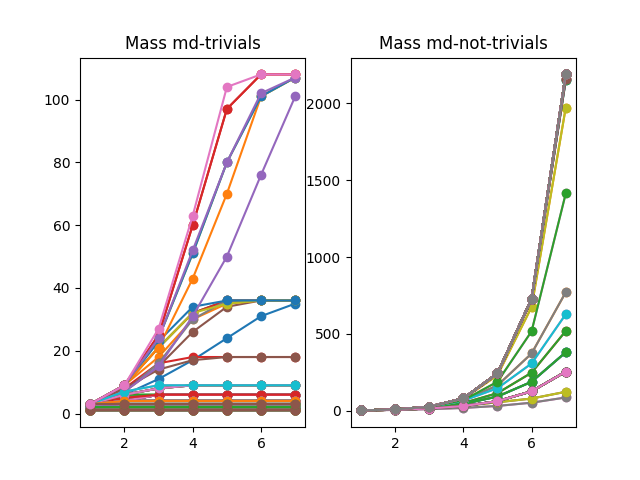
\includegraphics[width=\textwidth]{mass_33.png}
  \caption{Fonctions de croissance des automates à 3 états et 3 lettres $\mathfrak{md}$-triviaux à gauche et des non $\mathfrak{md}$-triviaux à droite.\label{fig:mass-33}}
\end{figure}

\begin{figure}[h]
  \centering
  % \includegraphics[width=\textwidth]{mass_53.png}
  \caption{Fonctions de croissance des automates à 5 états et 3 lettres $\mathfrak{md}$-triviaux à gauche et des non $\mathfrak{md}$-triviaux à droite.\label{fig:mass-53}}
\end{figure}

Nous en avons déduit que...

\subsection{Automates fantastiques}

Nous avons ensuite cherché dans des classes plus grandes que celles abordées jusqu'alors pour trouver des automates \textit{fantastiques}.

\begin{definition}
  Un automate est \textbf{\textit{fantastique}} s'il est $\mathfrak{mdc}$-trivial mais pas $\mathfrak{md}$-trivial.
\end{definition}

La factorisation est une opération coûteuse, pour tester la $\mathfrak{mdc}$-réduction il est donc préférable d'énumérer les classes de diviseurs et de faire tous les produits. On trouve ainsi tous les automates fantastiques d'une classe à isomorphisme près.

\begin{table}[h!]
  \begin{center}
    \begin{threeparttable}
      \begin{tabular}{|rrr|}
        \hline
        \#états & \#lettres & \#fantastiques \\ [0.5ex]
        \hline\hline
        \hline
        4 & 3 & 4 \\
        \hline
        4 & 4 & 38 \\
        \hline
        6 & 3 & 0 \\
        \hline
      \end{tabular}
      \caption{Nombre d'automates fantastiques pour des classes d'automates biréversibles}
    \end{threeparttable}
  \end{center}
\end{table}


Pour essayer de se convaincre que notre conjecture est correcte, il faut aussi s'assurer qu'aucun automate non $\mathfrak{mdc}$-trivial n'engendre du fini.

Nous avons donc considéré la borne supérieure du nombre d'états des $\mathfrak{m}(\mathcal{M}^5)$ où $\mathcal{M}$ est une machine biréversible à 4 états 3 lettres ou 4 états 4 lettres $\mathfrak{mdc}$-triviale puis vérifié que la fonction de masse des automates non $\mathfrak{mdc}$-triviaux dépasse bien cette borne. Bien que ce résultat ne prouve rien, il reste encourageant.


\section{Conclusions}

Nous n'avons pas réussi à décider si la $\mathfrak{mdc}$-réduction est un bon critère de finitude pour des classes d'automates plus grande qu'à 2 états ou 2 lettres.

Nous manquons encore d’outils pour pouvoir affirmer qu’un groupe engendre du fini ou non. Le problème étant indécidable en général cela n’est pas surprenant. La prochaine étape serait de chercher des critères de finitude analogues à la fonction de masse qui seraient plus efficaces, ou qui permettraient de réduire le nombre d'automates à traiter. L’étude de la fonction de masse seule est trop longue pour traiter des quantités d’automates comme celles que nous avons.

\newpage
\bibliography{project}{
  \nocite{*}
}
\bibliographystyle{plain}

\end{document}
